%%%%%%%%%%%%%%%%%%%%%%%%%%%%%%%%%%%%%%%%%%%%%%%%%%%%
%												   %
%                                   			   %
%   Antoine Faravelon, Lucas Felix,                %
%   Miratul Khusna Mufida, Hugo Guiroux,           %
%   Simon Moura                                    %
%												   %
%%%%%%%%%%%%%%%%%%%%%%%%%%%%%%%%%%%%%%%%%%%%%%%%%%%%

\documentclass[a4paper,10pt]{article}
\usepackage{amsthm}
\usepackage{amsmath}
\usepackage{amsfonts}
\usepackage{mathtools}
\usepackage{wrapfig}
\usepackage{graphicx}
\usepackage{titling}
\usepackage{float}
\usepackage{caption}
\usepackage{subcaption}
\usepackage{listings}
\usepackage{fullpage}
\lstset{%
    basicstyle=\scriptsize\sffamily,%
    commentstyle=\footnotesize\ttfamily,%
    frameround=trBL,
    frame=single,
    breaklines=true,
    showstringspaces=false,
    numbers=left,
    numberstyle=\tiny,
    numbersep=10pt,
    keywordstyle=\bf
}
\newcommand{\subtitle}[1]{%
    \posttitle{%
        \par\end{center}
    \begin{center}\large#1\end{center}
\vskip0.5em}%
}

\newcommand{\CCscript}[2]{
    \begin{itemize}
        \item[]\lstinputlisting[caption=#2,label=#1,language=CC]{src/#1.cc}
    \end{itemize}
}
\lstdefinelanguage{codeoutput} { %this is the name that you are going to use when you want to use the formatting
    basicstyle=\ttfamily\scriptsize, %font family & size
}
\newcommand{\Oscript}[2]{
    \begin{itemize}
        \item[]\lstinputlisting[caption=#2,label=#1,language=codeoutput]{src/#1}
    \end{itemize}
}
\newcommand{\Cscript}[2]{
    \begin{itemize}
        \item[]\lstinputlisting[caption=#2,label=#1,language=CC]{src/#1.c}
    \end{itemize}
}

\setlength{\abovecaptionskip}{1pt plus 1pt minus 1pt} % Chosen fairly arbitrarily

\title{Nachos}
\subtitle{Project [MOSIG - M1]}
\author{Antoine Faravelon, Lucas Felix, Miratul Khusna Mufida, Hugo Guiroux, Simon Moura}
\date{\today}

\begin{document}
\maketitle

\tableofcontents
\newpage

\section{Interesting/main features of our kernel}
    
\documentclass[a4paper,10pt]{article}
\usepackage{amsthm}
\usepackage{amsmath}
\usepackage{amsfonts}
\usepackage{mathtools}
\usepackage{wrapfig}
\usepackage{graphicx}
\usepackage{titling}
\usepackage{float}
\usepackage{caption}
\usepackage{subcaption}
\usepackage{listings}
\usepackage{fullpage}
\lstset{%
    basicstyle=\scriptsize\sffamily,%
    commentstyle=\footnotesize\ttfamily,%
    frameround=trBL,
    frame=single,
    breaklines=true,
    showstringspaces=false,
    numbers=left,
    numberstyle=\tiny,
    numbersep=10pt,
    keywordstyle=\bf
}
\newcommand{\subtitle}[1]{%
    \posttitle{%
        \par\end{center}
    \begin{center}\large#1\end{center}
\vskip0.5em}%
}

\newcommand{\CCscript}[2]{
    \begin{itemize}
        \item[]\lstinputlisting[caption=#2,label=#1,language=CC]{src/#1.cc}
    \end{itemize}
}
\lstdefinelanguage{codeoutput} { %this is the name that you are going to use when you want to use the formatting
    basicstyle=\ttfamily\scriptsize, %font family & size
}
\newcommand{\Oscript}[2]{
    \begin{itemize}
        \item[]\lstinputlisting[caption=#2,label=#1,language=codeoutput]{src/#1}
    \end{itemize}
}
\newcommand{\Cscript}[2]{
    \begin{itemize}
        \item[]\lstinputlisting[caption=#2,label=#1,language=CC]{src/#1.c}
    \end{itemize}
}

\setlength{\abovecaptionskip}{1pt plus 1pt minus 1pt} % Chosen fairly arbitrarily

\title{Nachos}
\subtitle{Project [MOSIG - M1]}
\author{Antoine Faravelon, Lucas Felix, Miratul Khusna Mufida, Hugo Guiroux, Simon Moura}
\date{\today}

\begin{document}

\section{Main Features Of The Program}


The nachos kernel offers most of the basic functionalities awaited from a kernel :\\
\begin{itemize}
\item synchronized Input/Output
\item User Multi Threading
\item Virtual memory and multiple processes running concurently
\item A file system
\item TCP/IP protocol
\end{itemize}

\subsection{A few interesting features}

First, all the the network functionalities have also been ported to the userspace. A user program can use sockets and 
transfer content other the network using the faclities offered by our nachos kernel. \\
We have also implemented the auto exit of the userthread so that, at the end of their execution, they do not return
into main code. And we can also catch their return values.\\
For this same threads, the kernel also give access to facilities to synchronize them (semaphore).\\
Processes have also been implemented with some managing functions. Indeed, though the kernel does not offer any 
processes hierarchy, a process can wait for the end of another one and then catch its exit value.\\
Also, in the userspace, we provide a minimal shell for use with our kernel. It provides a prompt and the ability
to launch program. Job management is also provided.\\
Finally, dynamic memory allocation has been implemented for the userspace. User can allocate \\dynamically on the heap 
instead of the stack.\\
After that, the user has access to a whole range of system calls that will be detailed in the following section.

\end{document}

\section{User documentation}
User documention has been moved in appendix for more lisibility.

\section{User test}
    \subsection{Motivation}
Testing has been an important phase in our whole development. In order to insure
that our implementation was still working after any changes, we made a lot of
regression tests. 

It means that, as soon as we added a new feature which was compiling, we were
able to check if it didn't generate any bugs or if it broke something we made before.

The idea was to create these tests in parallel with the implementation of new
parts of the kernel. Thus, we tried to test everything we implemented on top of
the given Nachos kernel.

\subsection{The way it works}
Our tests are divided in two directories, $regression$ and $test$. The
structure is the following :
\begin{itemize}
    \item $*.c$ files, in test directory, contains some programs which helped us
        test user-level features and system calls
    \item $x.desc$ files contains descriptions about the matching $x.sh$ scripts
    \item $x.sh$ are bash scripts calling either C programs or launching directly
        one nachos command line option
\end{itemize}


\subsection{How to run them}
To run all tests, just compile the kernel then enter the following command :
\textbf{make regression}.\\

It will run tests for all steps. Those which are marked as "ok" didn't raised
any error, the others did.\\

In order to not be lost while tests are running, we specified the step we were
working on at the beginning of the test name. For instance, $step5\_*$ tests are
related to file-system.\\

To create our tests we proceeded the following way :
\begin{itemize}
    \item First we create some basic test, as unitary as possible trying to
        cover each execution flow (including error handling)
    \item Then we create more complex tests using execution scenarios
\end{itemize}

We finally made $132$ tests for all nachos parts. 

\subsection{Examples}
\subsubsection{Consumers/Producers}
We implemented a producer/consumer test in user-mode using circular buffer.
We used two semaphores and one mutex. The mutex protects the critical section
where buffer is manipulated. The two semaphores are used as counter :
\begin{itemize}
    \item One for the number of empty slots inside buffer
    \item One for the number of currently available items inside buffer
\end{itemize}

We do this with five producers and five consumers with buffer of size three.

\subsubsection{The tiny shell}
A shell was implemented with jobs support. Program can be launched using
ForkExec.
These programs run either in foreground or background using \& at
the end of the command line.

The "jobs" command list all currently background running processes.

The "fg" command is used to switch a background process to foreground.

These tests allow to check ForkExec and WaitPid syscalls as well as processes
management.

\subsubsection{Stress process}
In the aim of testing our implementation limits on processes and threads, we
tried to create 150 processes, each of them with 40 threads.
It allows us to check if Nachos does not misbehave and handle limits properly.
Thus, running this test, we see that when the bounds are reached, bad request for
new process/threads creation are rejected.

%\begin{itemize}
%	\item GetChar() and PutChar()
%		\begin{itemize}
%		\item Basic Input Output character test
%		\item {\bf Test for character EOF}
%		\item {\bf Test for ASCII 255}
%		\end{itemize}
%	\item GetString() and PutString()
%		\begin{itemize}
%		\item Basic Input Output string test
%		\item {\bf Test for empty string}
%		\item {\bf Test for string EOF}
%		\item {\bf Test Maximum String}
%		\end{itemize}
%	\item GetInt() and PutInt()
%		\begin{itemize}
%		\item Basic Input Output Integer
%		\item {\bf Test Int EOF}
%		\item {\bf Test Int Everflow}
%		\end{itemize}
%\end{itemize} 
%
%\subsection{Part 3}
%
%3rd part implement threads and we provided such test the interesting one will mark as bold: 
%
%\begin{itemize}
%\item {\bf step3-multiple-join}
%\item {\bf step3-synchconsole-synch-put}
%\item {\bf step3-synchconsole-synch-rw}
%\item step3-synchconsole-synch
%\item {\bf step3-test-exit-delete-chilren}
%\item {\bf step3-test-recursive-threads-kill}
%\item {\bf step3-test-recursive-threads-simple}
%\item step3-threadArg
%\item step3-threadcreate
%\item step3-thread-exit-code-wait-too-late
%\item step3-thread-exit-delete-children
%\item step3-thread-exit
%\item {\bf step3-thread-join-after-join}
%\item step3-threadjoinerror
%\item {\bf step3-threadJoinMax}
%\item {\bf step3-threadJoinMultiple}
%\item step3-threadjoin
%\item step3-threadJoinSimple
%\item step3-thread-main-userthreadexit
%\item {\bf step3-thread-max-limit}
%\item {\bf step3-thread-Multiple-Kill-Create}
%\item {\bf step3-threadProdCons}
%\item step3-thread-return-code
%\item step3-threadSemaphore
%\item step3-thread-userthreadexit-function
%\item {\bf step3-use-destroyed-semaphore}
%\end{itemize} 
%
%\subsection{Part 4}
%
%This parts implement Memory Management and Process. We provided such test the interesting one will mark as bold :
%\begin{itemize}
%\item step4-fork-unknow-program
%\item {\bf step4-heap-alloc-free-behavior}
%\item {\bf step4-malloc-bad-free}
%\item step4-malloc-concurrent
%\item step4-malloc-free-multiple
%\item {\bf step4-malloc-just-fit}
%\item {\bf step4-malloc-multiple-process}
%\item step4-malloc-reuse-memory
%\item step4-malloc-simple 
%\item step4-malloc-will-fail
%\item {\bf step4-multiple-ForkExec}
%\item {\bf step4-Multiple-ForkExec-Waitpid} 
%\item step4-process-preempt
%\item step4-stress-process-thread
%\item step4-thread-Join-0
%\item {\bf step4-tiny-shell-test-extend}
%\item step4-tiny-shell-test
%\item {\bf step4-trigger-page-fault-multiple-process}
%\item step4-trigger-page-fault
%\item step4-userpages0
%\item step4-waitpid-return
%\end{itemize} 
%
%\subsection{Part 5}
%
%This parts implement FileSystem We provided such test the interesting one will mark as bold :
%\begin{itemize}
%\item step5-absolute-path
%\item {\bf step5-change-directory-kernel-one-thread}
%\item {\bf step5-change-directory-kernel-two-thread}
%\item step5-change-directory-simple
%\item step5-change-directory-thread
%\item {\bf step5-cp-verified}
%\item step5-create-directory-dot-dot-name
%\item step5-create-dot-name-file
%\item step5-create-dot-name
%\item step5-create-file-as-directory
%\item {\bf step5-create-file-bad-name}
%\item step5-create-file-dot-dot-name
%\item step5-create-file
%\item step5-create
%\item step5-directory-limit
%\item step5-directory-limit-third
%\item {\bf step5-directory-limit-with-files}
%\item {\bf step5-file-create-bad-name-directory}
%\item step5-file-create-directory-relative
%\item step5-file-create-directory
%\item step5-file-create-existing-directory
%\item {\bf step5-file-create-file-exist-directory}
%\item step5-file-create-file-relative
%\item step5-file-listing
%\item step5-fill-disk
%\item step5-listing-directory-one-level-second
%\item step5-listing-directory-one-level
%\item step5-listing-directory-relative
%\item step5-listing-directory-simple
%\item {\bf step5-max-file-open-fork}
%\item step5-max-file-open-simple
%\item step5-max-file-open-thread
%\item step5-multiple-file-open
%\item {step5-open-file-table-rw}
%\item step5-open-same-file-process
%\item step5-recursive-listing
%\item {\bf step5-remove-existing-empty-directory-first}
%\item {\bf step5-remove-existing-empty-directory-last}
%\item {\bf step5-remove-existing-empty-directory-middle}
%\item step5-remove-file
%\item step5-remove-non-existing-directory
%\item step5-remove-opened-file
%\item {\bf step5-remove-recreate-directory}
%\item step5-remove-relative-path
%\item step5-remove-root
%\item {\bf step5-rw-concurrent-read}
%\item step5-seek
%\item step5-thread-close-read
%\item step5-threads-open-write-read-close
%\item step5-threads-write
%\item {\bf step5-too-big-file}
%\item {\bf step5-too-large-file}
%\item {\bf step5-two-thread-opening-file}
%\end{itemize} 
%
%\subsection{Part 6}
%
%This parts implement Network. We provided such test the interesting one will mark as bold :
%\begin{itemize}
%\item {\bf step6-multiple-listen-same-port}
%\item step6-receive-message-waiting
%\item step6-send-message-not-connected
%\item step6-simple-listen-connect-accept
%\item step6-test-accept-failed
%\item step6-test-incomplete-acknowledgement
%\item {\bf step6-test-big-message}
%\item {\bf step6-test-multithread}
%\end{itemize} 

\section{Implementation choices}
    \subsection{Synchronized Console}

For consistency inside outputs, we needed to implement synchronization
mechanisms. To do that, we choose to use the \textbf{Monitor} concurrent
programming model.\\
Each methods of the synchconsole was encapsulated using two
semaphores :
\begin{itemize}
    \item one for read \textbf{read} (GetInt, GetString, GetChar)
    \item one for \textbf{write} (PutInt, PutString, PutChar).
\end{itemize}

As GetString/GetInt and PutString/PutInt call respectively GetChar and PutChar,
we either need recursive semaphores or make internals sub-routines
\_GetChar/\_PutChar which are called by GetString/GetInt/GetChar, letting the
synchronization mechanism inside these calling methods.\\
The second choice was made for simplicity.\\

To conclude with synchronized console implementation choices, we had to handle
error inside GetChar and GetInt :
\begin{itemize}
    \item For GetChar, the choice was made to return an integer instead of a char. By
convention, \textbf{EOF} is $-1$.
    \item For GetInt, we cannot used a long int because the return value of a syscall is
inside a register which is of size $4$. Thus the address of an int is needed by
GetInt. This int will be filled with the getting number and the return value of
GetInt is used to handle error (see user documentation for more information).
\end{itemize}

\subsection{Multi-Threads}

Concerning stacks management, the first kernel thread (created at \emph{Nachos}
start) use the UNIX-process stack. Other kernel threads use heap-allocated
stacks. For user thread, each thread as his own stack, from bottom of the memory
up to the top. All user thread stacks are handled inside StackMgr class.
StackMgr handle all stacks requests inside a AddrSpace. If UserThreadCreate is
called and no space for stack is available, the function returns $-1$.\\

A word about thread hierarchy. There is none. This mean that every thread
belongs to a process. A thread can create other threads but the behavior (e.g
exit) does not influence others.

A user thread can exit in two ways :
\begin{itemize}
    \item calling \textrm{UserThreadExit(void *ret)} where $ret$ is a generic
        pointer to the returned data
    \item returning from the thread function (also a generic pointer)
\end{itemize}

%One exception is for the first thread (the one with the main function). As
There is an exception for the first thread (the one with the main function). As
pthread implementation, calling \textrm{UserThreadExit} with main thread let
other threads finish. After the last thread end, it will exit the process.\\

As threads are light-weight processes, calling \textrm{Exit} in any threads
kill the process with all threads belonging to it. This is the same if the main
thread reach the return of the main function. It will implicitly call
\textrm{Exit}. Thus does not wait for threads termination.\\

It is noticeable that thread id (tid) are unique to a process during is
lifetime. A tid will never be re-used. This allows us to implement
\textrm{UserThreadJoin} as discussed below.

\textrm{UserThreadJoin(unsigned int tid, void **retval)} allows one thread to wait for
another.\\
Inside retval (if not NULL) you can get the value return either by
\textrm{UserThreadExit} or by the return value of thread function. If that
thread has already terminated, then \textrm{UserThreadExit} returns
immediately.\\
If multiple threads simultaneously try to join with the same thread, only the
first one will be able to join on it. For others, syscall will return error
code $-2$. \\
If threads join multiple times on the same thread (not at the same time), each
call will be successful and if retval is not NULL, it will be filled with the
return value of thread.\\

About semaphores, they are now available to user program using
UserSemaphoreCreate syscall. This return a semaphore id process-specific. To
wait for resource being available, \textrm{UserSemaphoreP} is here. To notify resource
availability, it's\textrm{ UserSemaphoreV}. Finally,\textrm{ UserSemaphoreDestroy} destroys a
semaphore. Semaphore id are process-unique and not re-used. If a
UserSemaphore[P|V] is used after the semaphore was destroyed, these syscalls
will return $-1$. All semaphores are destroyed at the end of a process.

\subsection{Virtual Memory}

To handle virtual memory, all requests for memory page allocation/deallocation
was made through a FrameProvider. This component has his own frame placement
policy. Everytime a process (via his AddrSpace) ask the FrameProvider for
physical pages when it is needed (for Stack, Heap or Code/Data segments).
We implemented different strategies to see if our model was coherent : random,
first and last.\\

A heap management was implemented. Stack and heap have fixed max size and
we let a page between both in order to throw a page fault we try to access
outside the bounds. A HeapMgr which embed a top heap pointer manage requests for
new heap pages.
Heap and stack pages are dynamically allocated using FrameProvider.

\subsection{Multi-Processes}
ForkExec creates new kernel thread that will execute new user program in a new
address space. The creation of the new process is divided between the calling
thread and the called thread which will begin its execution with a special
initialization function. The managing of the processes is done by the processMgr
object which manages the pids and the ability to wait for a certain thread using
Waitpid function.\\

There is no processes hierarchy, only the number of currently running threads is
counted and when the last process exit the machine is halted.

When a process halt it does not affect the others since all are independent
programs with their own virtual memory code, data, and stacks.\\

Each pid is unique so when using Waitpid it is possible to know and prevent the
process from waiting on a dead process or on itself. And as such it is possible
to avoid deadlocks that would happen otherwise.

Waitpid allows to catch the exit code of the process which is being waited.

\subsection{FileSystem}
For Filesystem, we followed the subject.

\subsubsection{Sub-Directory and Current Directory}

We added an attribute inside the directory table. This attribute ($isDir$) allows
to distinguish between files and directory. A function called
\textrm{ExpandFilename} handle all ``.'', ``..'' to compute the absolute
path. This allows us to avoid creating two special files inside each directory,
saving two entries.\\

A notion of CurrentDirectory was implemented attached to a process. Each process
has his own directory and relative path are computed taking into account this
one. All paths are computed using ExpandFilename.

\subsubsection{Open file table}
Each process has his own file table which is typically a unique identifier and a
FileInfo structure. This file structure allows checking which thread own the
file, which file name was already opened to apply some restrictions.

\subsubsection{Max File Size and Dynamic Size}
By default, each file was limited to $\frac{SectorSize - 2*4)}{4} * SectorSize$
bytes ($3.75K$). Either the $SectorSize$ needs to be extended, or another
indirection level was added.
Now the $\frac{SectorSize - 2*4}{4}$ data sectors of a FileHdr points to
DataBlockHdr. Each of these DataBlockHdr points to $\frac{SectorSize}{4}$ data
block (the real content).
The maximum size is now of $(\frac{SectorSize - 2*4}{4} +
\frac{SectorSize}{4})*SectorSize$ bytes ($122kB$).\\

When a file is created, it has a size of $0$. At each write, if needed, file size is
expanded allocating Data Sector and DataBlock sector.

\subsubsection{Concurrent Accesses}
The SynchFileMgr component manages all concurrent accesses to a same file
(represented by the sector of his FileHdr). Attached to this sector, a
ReaderLock and a WriterLock are used for implementing a reader/writer schema for
all file accesses across all processes and threads.

\subsection{Network}
We chose to implement a socket user interface in our Nachos kernel. These
sockets work in connected mode with robust transmissions.\\
As in TCP sockets, a server create a listening socket and accept new
connections on it. This allow to join a server on one port (defined by
convention as $80$ for HTTP servers) with many clients, and each of them will then
have a personal socket with the server.
On its side, the server can communicate with each client separately on
different sockets. Our kernel provides $16$ ports which can handle $16$ sockets
each, so the kernel can handle $256$ connections at a time.

\subsection{Low level transmission}
The lower layer of our network implementation is the transmission of one mail.
This part have to be robust and then we can construct an higher level protocol
on it.\\
For every single mail, the emitter send the mail, wait a confirmation and retry
if no. The number of tries is limited and the send function will return an
error if this limit is reached.
The receiver can receive many times the same mail before the emitter receive a
confirmation. To prevent the duplication of a mail, we include an id in each of
them. The receiver will take the first iteration of a mail and just confirm the
other. The id we use is an int which is always incremented, so the socket will stop
to work after $2^{32}$ mails sent. This limit is hard to reach, so we did not
deal with it, but it is possible to make the id go back to $0$ when it happens
without blocking the network.
A confirmation mail contains the id of the mail it confirm, so a confirmation
mail cannot be used later by the emitter to confirm an other mail.

\subsection{Protocol}
Then we constructed the connected protocol over the robust transmission.
The connection establishing use a three-way handshake.\\
We use the mailboxes of the initial Nachos code as ports, but now each mailbox contains an array of 
socket because many sockets can be connected within a same port (for instance the
port $80$ of HTTP servers).  The number of connections a port can handle is limited 
to $16$, because an array was simpler to implement and $16$ is sufficient (but it 
can be replaced easily by a list).\\
The postal worker dispatch the mails he receive. He know in which mailbox
thanks to the mail header and then find the good socket by comparing the origin
of the mail to the ones contained into sockets.\\
Here is the schema of the classes used in network :
\begin{figure}[H]
	\centering
		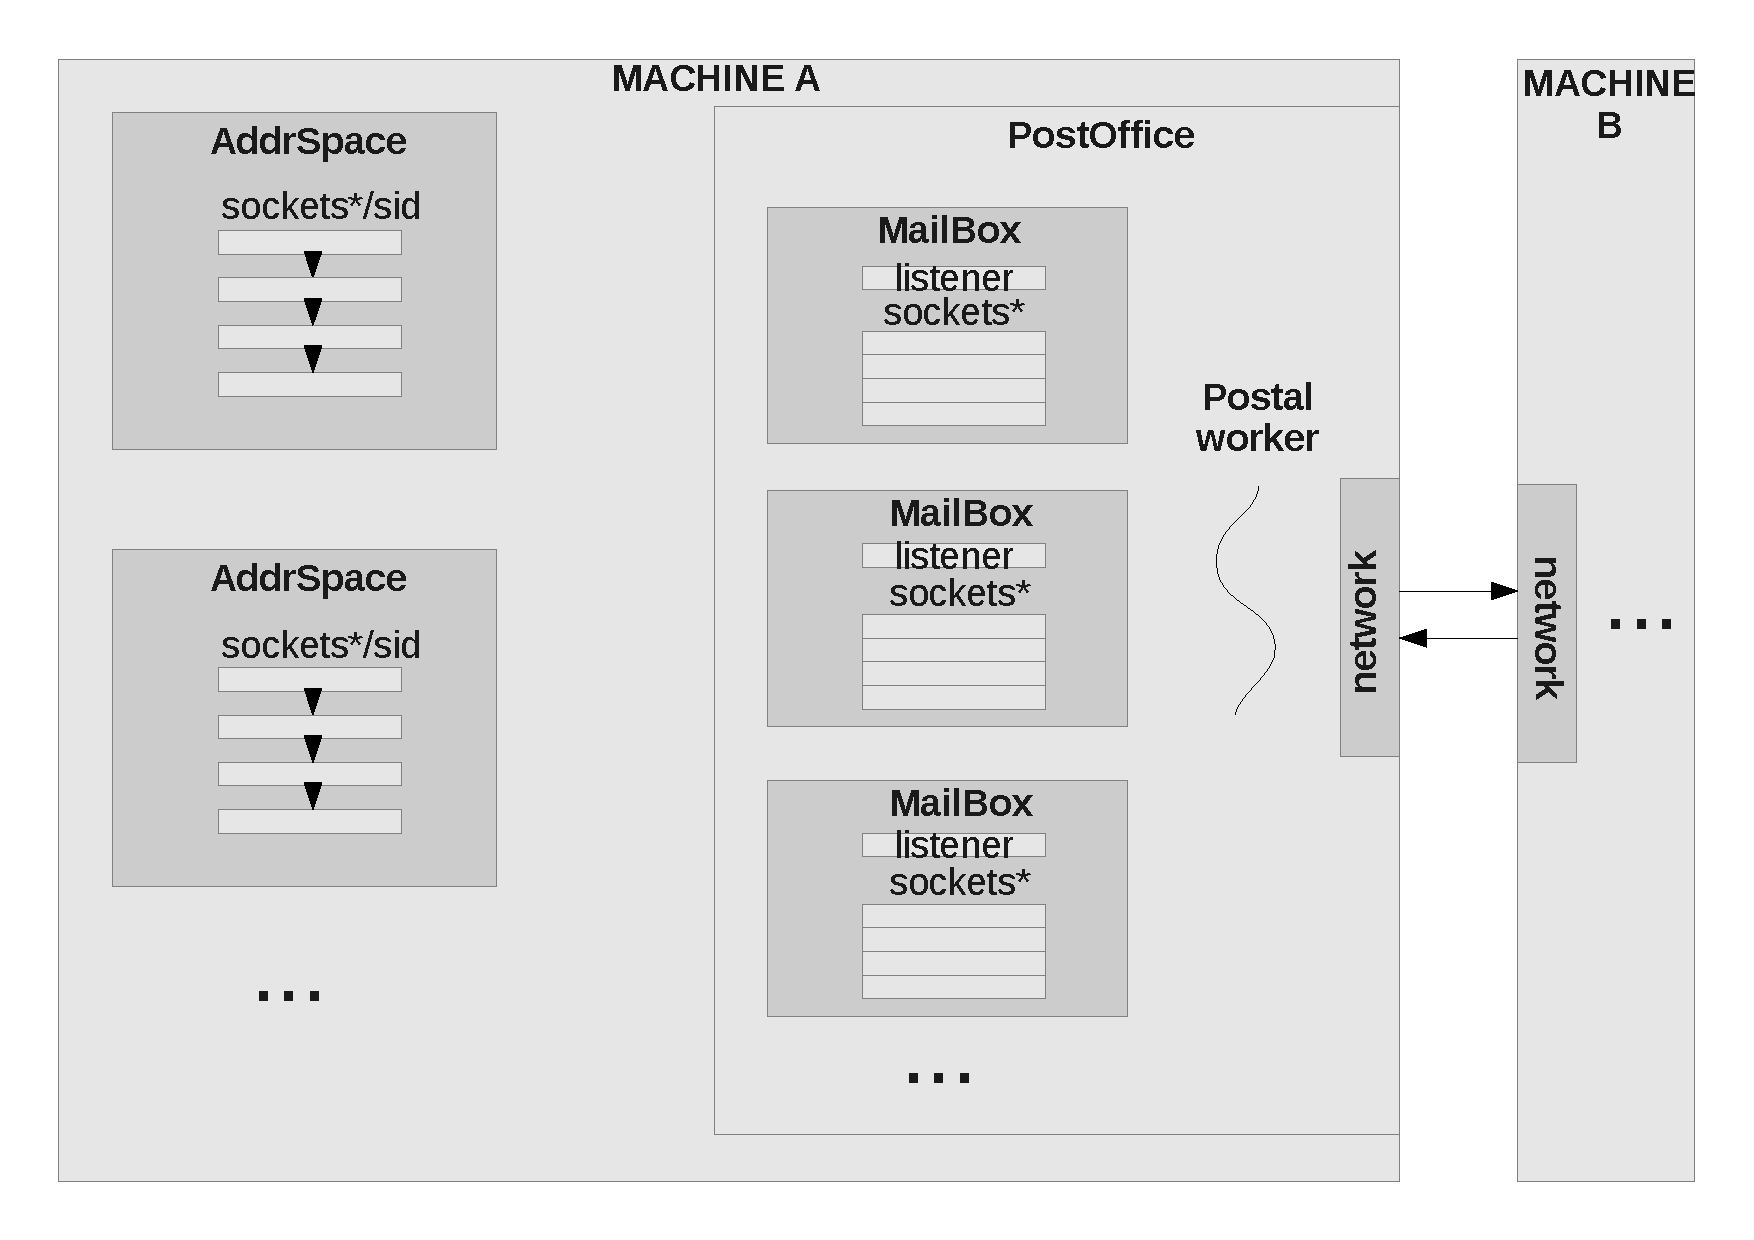
\includegraphics[scale=0.4]{networkschema}
		\caption{Each socket can be accessed from its address space and the mailbox which handle it.}
\end{figure}
%%% Local Variables:
%%% mode: latex
%%% TeX-master: "report_nachos"
%%% End:


\section{Organization}
    \subsection{Implementation}
First we decided to work everyday at the university so as to make communication between members of the group easier.
Allowing us to solve bug faster, avoid derivation from the specification and cut the wok dynamically(reevaluate 
planning in real time when need be).\\
For each step, before begining anything, we would all read and understand the subject. Then discuss with each other,
establish a todo list and then we would distribute the work. \\ 
Then, during the implementation, we would often make summary of our work to explain the implementation of every part 
of the code to the rest of the group.\\
To make the group work easier we used a git repository. This allowed us to share our work more efficiently as code
this tool can manage code merges automatically or at least make them easier. And allow us to work even when not
at the university and still be able to share the code immediately if need be.\\

\subsection{Validation}
Following the principle of the test driven development a large set of automated regression tests were developped. 
It was used to validate the code or point out one or multiple bug / regressions in it in a comfortable, fast
way and easily understandable way. \\
A failure on a test will indicate what the test was about, thus allowing us to point out the error easily.And by 
doing the test before or during the implementation this automated tests can allow to esily monitor the state and the
advancement of the part currently being implementated.\\ Indeed During the begining of the  implementation, one of 
the members would implement the tests while the other began coding wich allows to have tests ready as soon as the 
program compiles. \\
Valgrind has also been extensively used to remove memory leaks and unsafe memory access. Thus suppressing a 
signicative number of possible bugs in the program. The program should now be free of any illegal memory access
and memory leak.

\subsection{Part 1 to 4}

For the parts 1 to 4, we followed the subject and all worked on the same part. We usually split into two teams.
Splitting the works of the whole step into two main parts. In this teams, we practiced extrem programing so as to
compensate for the fact that all the work could not easily be split between each member. . Thus making the debugging phase faster. During the complicated phases,
having two persons working on the same problem often allowed us to solve it faster and to avoid many bugs in the code
that a single person would not notice while coding.\\
Also, when working in pair (or triple) the tests were not done by the person who was currenty coding, thus they 
were not made with the weakness of the program in mind and tested uniformly the program without sparing some part 
or another.

\subsection{Part 5 and 6}

The parts 5 and 6 were done in parallel. The group was separated in two teams, each team working on one step.
For the rest, the same philosophy as for the first parts was applied. That is, each team worked following the
extreme programing principle.\\
The git repository was split in two working branches to make the work easier for both team as the two part were
independant but required to work in the same files thus causing unescessary conflicts and possibly bugs that would
disturb the team not causing them. We used tags to separate these two branches.

\subsection{Last two days}

On the last days, one person took care of the merging of the two branches. The other made a Todo List for the report 
and presentation, then everyone took one part of it to prepare. 


\section{Conclusion}
    There still exists some unimplemented functions in our kernel due to lack of
time.\\ 
For the network, the migration of process and thread safe sockets have
yet to be implemented. The process migration is still to be defined, but the
sockets just miss the actual implementation of the necessary locks.\\
For the file-system, the optimization of input/output and robustness were not
implemented.\\
In an other hand, thanks to the regression test, it is possible to say that, a
priori, every implemented part should be working. Though the set of test can
not be completed and as such it is still possible that there is still exists bugs
that were not tested.\\


\appendix
    \subsection{Syscalls}
\begin{description}
    \item [NAME] : \textbf{halt}
        \begin{itemize}
            \item SYNOPSIS : void Halt()
            \item DESCRIPTION :
                Halt is a system call which power off the system.
        \end{itemize}


    \item [NAME] : \textbf{Exit}
        \begin{itemize}
            \item SYSNOPSIS : void Exit(int status)
            \item DESCRIPTION :
                The exit syscall is used to quit the process. It will not shut down the
                machine unless there is no other process running.
        \end{itemize}

    \item [NAME] : \textbf{PutChar}
        \begin{itemize}
            \item SYSNOPSIS : void PutChar(char c)
            \item DESCRIPTION :
                PurtChar is a function which will write the character c to the console.
        \end{itemize}

    \item [NAME] : \textbf{GetChar}
        \begin{itemize}
            \item SYSNOPSIS : int GetChar()
            \item DESCRIPTION :
                GetChar is a function that read a character from the input buffer.
            \item RETURN :
                \begin{itemize}
                    \item The character itself or EOF if there is none in the buffer
                \end{itemize}
        \end{itemize}

    \item [NAME] : \textbf{PutInt}
        \begin{itemize}
            \item SYSNOPSIS : void PutInt(int i)
            \item DESCRIPTION :
                PutInt is a function which is used to write the integer i to the console.
        \end{itemize}

    \item [NAME] : \textbf{GetInt}
        \begin{itemize}
            \item SYSNOPSIS : int GetInt(int* p)
            \item DESCRIPTION :
                GetInt read an integer from the input buffer pointed out by p.
            \item RETURN :
                \begin{itemize}
                    \item 0 if there is no error
                    \item -1 when the input cannot be read as an int
                    \item -2 when the address p cannot be written by the caller
                \end{itemize}
        \end{itemize}

    \item [NAME] : \textbf{PutString}
        \begin{itemize}
            \item SYSNOPSIS : void PutString(const char s[])
            \item DESCRIPTION :
                PutString writes the string $s$ to the console. If the string given is longer than
                MAX\_STRING\_SIZE then the remaining part is not printed in the console.
        \end{itemize}

    \item [NAME] : \textbf{GetString}
        \begin{itemize}
            \item SYSNOPSIS : char *GetString(char *s, int n)
            \item DESCRIPTION :
                It reads at most $n-1$ characters in the console.
            \item RETURN :
                \begin{itemize}
                    \item $s$ if there is no error
                    \item otherwise return NULL (in case of error or EOF)
                \end{itemize}
        \end{itemize}

    \item [NAME] : \textbf{UserThreadCreate}
        \begin{itemize}
            \item SYSNOPSIS : int UserThreadCreate(void f(void *arg), void *arg)
            \item DESCRIPTION :
                This function create a new thread which will execute the function f with the
                argument arg.
            \item RETURN :
                \begin{itemize}
                    \item 0 on success
                    \item -1 if no space left for stack
                    \item -2 if MAX\_TOTAL\_THREADS (20 by default) has been reached
                \end{itemize}
        \end{itemize}


    \item [NAME] : \textbf{UserThreadExit}
        \begin{itemize}
            \item SYSNOPSIS : void UserThreadExit(void *ret)
            \item DESCRIPTION :
                This function is used to destroy the current thread and puts the return value in
                $ret$.
                When the main thread call UserThreadExit, other threads continue to
                run. The last thread to end will call Exit.
                When a thread function reach a return statement, it will be converted
                to this syscall with return value as argument.
        \end{itemize}

    \item [NAME] : \textbf{UserThreadJoin}
        \begin{itemize}
            \item SYSNOPSIS : int UserThreadJoin(int tid, void **retval)
            \item DESCRIPTION :
                This function is used to join another thread (eg : wait for the tread
                of tid $tid$ to terminate). If multiple threads tries to join on the same
                thread, only the first one will be able to join on it. The function
                will return an error for the others.
                If retval is not null, it contains the return value of exit thread,
                either by calling UserThreadExit or by reaching the end of thread function.
            \item RETURN :
                \begin{itemize}
                    \item 0 on success
                    \item -1 if bad tid
                    \item -2 if another thread is already joining on the same thread tid
                \end{itemize}
        \end{itemize}

    \item [NAME] : \textbf{UserSemaphoreCreate}
        \begin{itemize}
            \item SYSNOPSIS : int UserSemaphoreCreate(char* name, int value)
            \item DESCRIPTION :
                Initialize and return a semaphore id named "name" with an initial value "value".
                It do not create a semaphore with the id of a previously destroyed semaphore.
            \item RETURN :
                \begin{itemize}
                    \item Return the id of the semaphore freshly created
                \end{itemize}
        \end{itemize}

    \item [NAME] : \textbf{UserSemaphoreP}
        \begin{itemize}
            \item SYSNOPSIS : int UserSemaphoreP(int id)
            \item DESCRIPTION :
                Takes the lock on the semaphore pointed by id.
            \item RETURN :
                \begin{itemize}
                    \item 0 on success
                    \item -1 if error (semaphore does not exist)
                \end{itemize}
        \end{itemize}

    \item [NAME] : \textbf{UserSemaphoreV}
        \begin{itemize}
            \item SYSNOPSIS : int UserSemaphoreV(int id)
            \item DESCRIPTION :
                Release the lock (unlock) the semaphore pointed by id.
            \item RETURN :
                \begin{itemize}
                    \item 0 on success
                    \item -1 if error (semaphore does not exist)
                \end{itemize}
        \end{itemize}

    \item [NAME] : \textbf{UserSemaphoreDestroy}
        \begin{itemize}
            \item SYSNOPSIS : int UserSemaphoreDestroy(int id)
            \item DESCRIPTION :
                Destroy the semaphore pointed by id.
            \item RETURN :
                \begin{itemize}
                    \item 0 on success
                    \item -1 if error (semaphore does not exist)
                \end{itemize}
        \end{itemize}

    \item [NAME] : \textbf{AllocPageHeap}
        \begin{itemize}
            \item SYSNOPSIS : int AllocPageHeap()
            \item DESCRIPTION :
                AllocPageHeap asks for a new page on heap.
            \item RETURN :
                \begin{itemize}
                    \item -1 if no more page for heap
                    \item new page $addr$ otherwise
                \end{itemize}
        \end{itemize}

    \item [NAME] : \textbf{FreePageHeap}
        \begin{itemize}
            \item SYSNOPSIS : int FreePageHeap()
            \item DESCRIPTION :
                FreePageHeap gives back a new page for heap.
            \item RETURN :
                \begin{itemize}
                    \item The new heap top $addr$
                \end{itemize}
        \end{itemize}

    \item [NAME] : \textbf{ForkExec}
        \begin{itemize}
            \item SYSNOPSIS : unsigned int ForkExec(char *s)
            \item DESCRIPTION :
                ForkExec creates a new process that execute the program stated in the argument $s$.
            \item RETURN :
                \begin{itemize}
                    \item pid of the newly created process in case of creation success
                    \item -1 if more than MAX\_PROCESS processes have been created (by default 30)
                    \item -2 case of an invalid executable
                \end{itemize}
        \end{itemize}

    \item [NAME] : \textbf{Waitpid}
        \begin{itemize}
            \item SYSNOPSIS : int Waitpid(unsigned int pid, int *retval)
            \item DESCRIPTION :
                Waitpid wait on the process which pid is given as argument.
                If $retval$ not NULL, the exit code of the process is put at address $retval$.
            \item RETURN :
                \begin{itemize}
                    \item -1 if process does not exist
                    \item -2 if process is dead
                    \item -3 if waiting for itself
                    \item 0 otherwise
                \end{itemize}
        \end{itemize}

    \item [NAME] : \textbf{Open}
        \begin{itemize}
            \item SYSNOPSIS : int Open(const char* filename)
            \item DESCRIPTION :
                Open try to open file *filename* taking into account current directory,
                returning a unique identifier
            \item RETURN :
                \begin{itemize}
                    \item -1 if file can not be opened
                    \item -2 if MAX\_OPEN\_FILES (default 10) are already opened
                    \item -3 if the file is already opened by another thread/process
                    \item id $\in [0; MAX\_OPEN\_FILES[$ a unique identifier used for future syscall
                        \end{itemize}
                \end{itemize}

            \item [NAME] : \textbf{Close}
                \begin{itemize}
                    \item SYSNOPSIS : int Close(int id)
                    \item DESCRIPTION :
                        Close try to close file with identifier *id*.
                    \item RETURN :
                        \begin{itemize}
                            \item -1 if file $id$ does not exists
                            \item 0 otherwise
                        \end{itemize}
                \end{itemize}

            \item [NAME] : \textbf{Create}
                \begin{itemize}
                    \item SYSNOPSIS : int Create(const char *filename)
                    \item DESCRIPTION :
                        Create file $filename$ taking into account current directory.
                    \item RETURN :
                        \begin{itemize}
                            \item -1 if creation failed
                            \item 0 otherwise
                        \end{itemize}
                \end{itemize}

            \item [NAME] : \textbf{Read}
                \begin{itemize}
                    \item SYSNOPSIS : int Read(int id, char *buffer, int numBytes)
                    \item DESCRIPTION :
                        Try to read $numBytes$ inside file $id$ and store result in $buffer$.
                        $buffer$ should be large enough to fit $numBytes$.
                    \item RETURN :
                        \begin{itemize}
                            \item -1 if file does not exists
                            \item other $numReadBytes$ the real number of bytes read
                        \end{itemize}
                \end{itemize}

            \item [NAME] : \textbf{Write}
                \begin{itemize}
                    \item SYSNOPSIS : int Write(int id, const char* from, int numBytes)
                    \item DESCRIPTION :
                        Try to write inside file $id$ at most $numBytes$ bytes stored in $from$
                        memory.
                    \item RETURN :
                        \begin{itemize}
                            \item -1 if the file does not exists
                            \item otherwise $numWriteBytes$ the real number of bytes
                        \end{itemize}
                \end{itemize}

            \item [NAME] : \textbf{Seek}
                \begin{itemize}
                    \item SYSNOPSIS : int Seek(int id, int position)
                    \item DESCRIPTION :
                        Move at position $position$ inside file $id$ relative to the beginning of
                        the file.
                    \item RETURN :
                        \begin{itemize}
                            \item -1 if the file does not exists
                            \item 0 otherwise
                        \end{itemize}
                \end{itemize}

            \item [NAME] : \textbf{Remove}
                \begin{itemize}
                    \item SYSNOPSIS : int Remove(const char* name)
                    \item DESCRIPTION :
                        Delete file named $name$.
                    \item RETURN :
                        \begin{itemize}
                            \item -1 if the file does not exists
                            \item -2 if the file is opened by another process
                            \item 0 otherwise
                        \end{itemize}
                \end{itemize}

            \item [NAME] : \textbf{GetCurrentDirectory}
                \begin{itemize}
                    \item SYSNOPSIS : char *GetCurrentDirectory(char *result)
                    \item DESCRIPTION :
                        Write the current process directory (absolute path) inside buffer $result$.
                    \item RETURN :
                        \begin{itemize}
                            \item address of $result$ (never fail, can be ignored)
                        \end{itemize}
                \end{itemize}

            \item [NAME] : \textbf{SetCurrentDirectory}
                \begin{itemize}
                    \item SYSNOPSIS : int SetCurrentDirectory(const char* dirname)
                    \item DESCRIPTION :
                        Set the current directory to $dirname$ of current process.
                        $dirname$ can be relative path to current directory.
                    \item RETURN :
                        \begin{itemize}
                            \item -1 if dirname does not exists
                            \item 0 otherwise
                        \end{itemize}
                \end{itemize}
        \end{description}


\subsection{Malloc}
  An implement of malloc/free as been provided as on UNIX. realloc and calloc
  are also available.

  Same rules and same prototypes as for UNIX version (see man malloc). Our
  version dynamically allocate and release pages for heap.

  In context of multithreads, you need to call memory\_init into the main thread
  before forking thread to initialize synchronization structure. This is not
  needed (but not wrong) for no-thread applications (only the main thread).

  Three allocations strategy has been implemented :
  \begin{itemize}
  \item FIRST\_FIT
  \item BEST\_FIT
  \item WORSE\_FIT
  \end{itemize}
  To use this library, include at top of your program :

  \begin{lstlisting}[language=C]
    #define BEST_FIT 1 
    #include "mem_alloc.c"
  \end{lstlisting}
  By default, the strategy is FIRST\_FIT and the first line (define) is
  unnecessary. The mem\_alloc.*c* is needed as Makefile only compile one file as
  a binary.

\end{document}
